%%% template.tex
%%%
%%% This LaTeX source document can be used as the basis for your technical
%%% paper or abstract. Intentionally stripped of annotation, the parameters
%%% and commands should be adjusted for your particular paper - title, 
%%% author, article DOI, etc.
%%% The accompanying ``template.annotated.tex'' provides copious annotation
%%% for the commands and parameters found in the source document. (The code
%%% is identical in ``template.tex'' and ``template.annotated.tex.'')

\documentclass[conference]{acmsiggraph}

\TOGonlineid{45678}
\TOGvolume{0}
\TOGnumber{0}
\TOGarticleDOI{1111111.2222222}
\TOGprojectURL{}
\TOGvideoURL{}
\TOGdataURL{}
\TOGcodeURL{}

\title{3D Printing for Mobile Robots}

\author{Andrew Spielberg\thanks{e-mail:aespielberg@csail.mit.edu} \and Vicki Crosson\thanks{e-mail:viccro.mit@gmail.com}}
\pdfauthor{Andrew Spielberg and Vicki Crosson}

\keywords{3D Printing, Robotics, 3Doodler, Trajectory Controller}

\begin{document}

%% \teaser{
%%   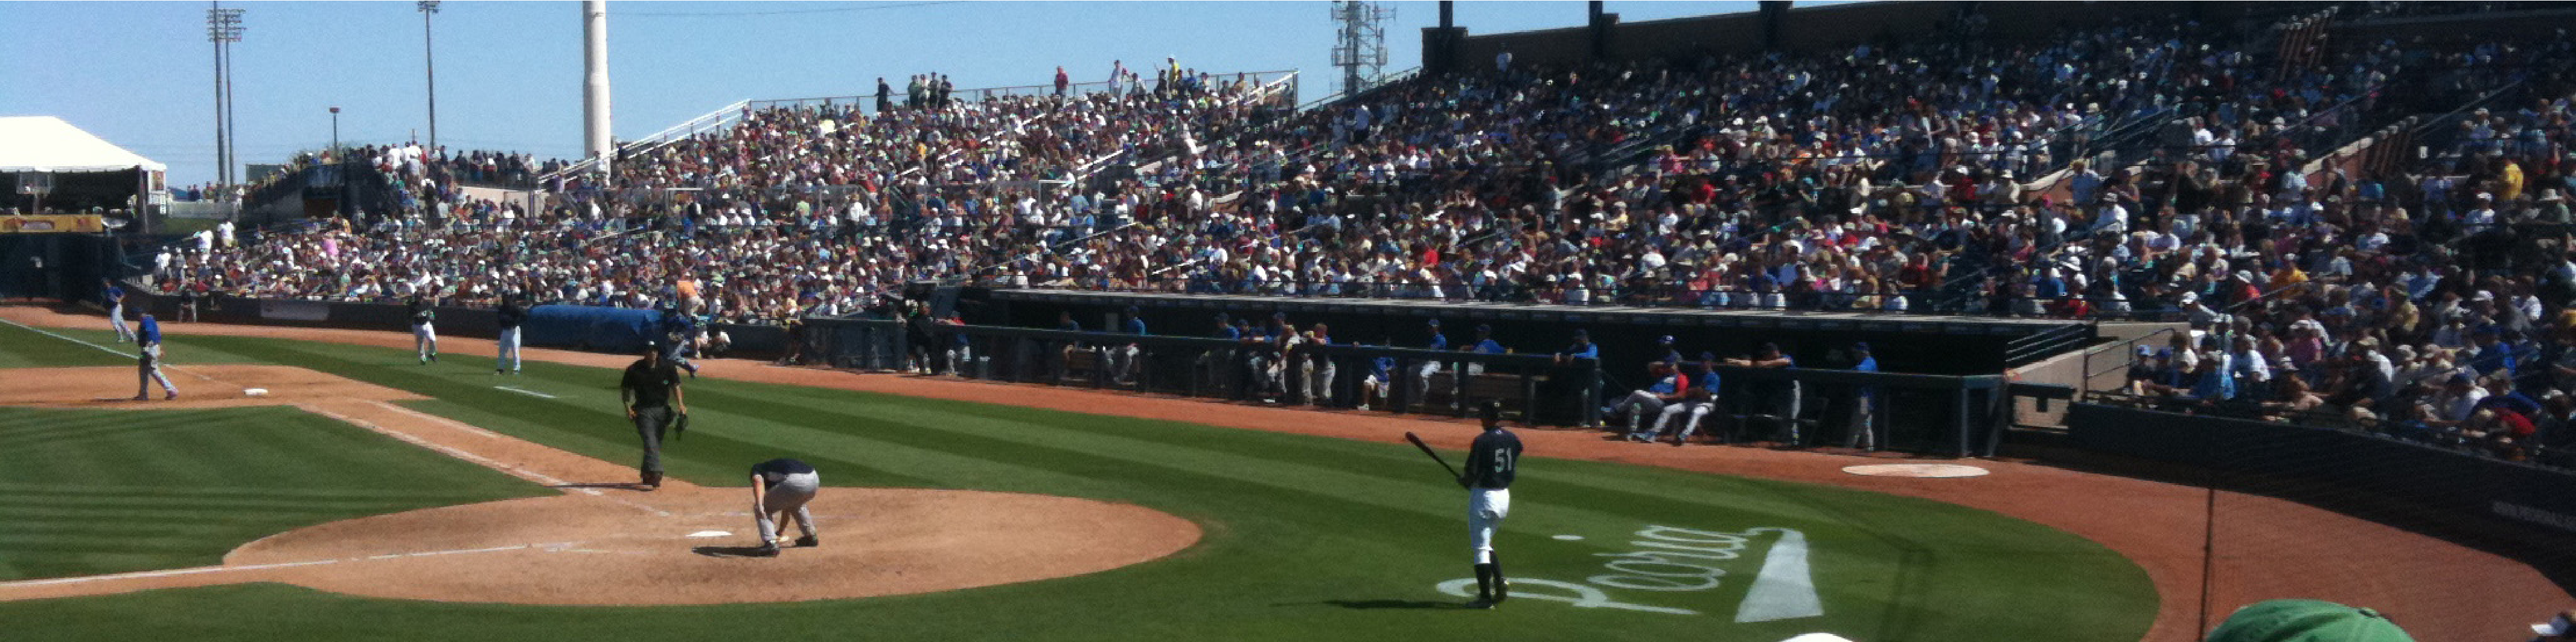
\includegraphics[height=1.5in]{images/sampleteaser}
%%   \caption{Spring Training 2009, Peoria, AZ.}
%% }

\maketitle

\begin{abstract}

Duis autem vel eum iriure dolor in hendrerit in vulputate velit esse
molestie consequat, vel illum dolore eu feugiat nulla facilisis at 
vero eros et accumsan et iusto odio dignissim qui blandit praesent
luptatum zzril delenit augue duis dolore te feugait nulla
facilisi. Lorem ipsum dolor sit amet, consectetuer adipiscing elit,
sed diam nonummy nibh euismod tincidunt ut laoreet dolore magna
aliquam erat volutpat.

Citations can be done this way~\cite{Jobs95} or this more concise 
way~\shortcite{Jobs95}, depending upon the application.

Ut wisi enim ad minim veniam, quis nostrud exerci tation ullamcorper
suscipit lobortis nisl ut aliquip ex ea commodo consequat. Duis autem
vel eum iriure dolor in hendrerit~\cite{Pellacini:2005:LAH}
in vulputate velit esse molestie~\cite{notes2002} 
consequat, vel illum dolore eu feugiat nulla facilisis at vero eros et
accumsan et iusto odio dignissim qui blandit praesent luptatum zzril
delenit augue duis dolore te feugait nulla facilisi.~\cite{Park:2006:DSI}

\end{abstract}

%\begin{CRcatlist}
%  \CRcat{I.3.3}{Computer Graphics}{Three-Dimensional %Graphics and Realism}{Display Algorithms}
%  \CRcat{I.3.7}{Computer Graphics}{Three-Dimensional %Graphics and Realism}{Radiosity};
%\end{CRcatlist}

\keywordlist

%% Use this only if you're preparing a technical paper to be published in the 
%% ACM 'Transactions on Graphics' journal.

\TOGlinkslist

%% Required for all content. 

\copyrightspace

\section{Introduction}


\begin{equation}
 \sum_{j=1}^{z} j = \frac{z(z+1)}{2}
\end{equation}

\begin{eqnarray}
x & \ll & y_{1} + \cdots + y_{n} \\
  & \leq & z
\end{eqnarray}


\section{System Overview}


\begin{figure}[ht]
  \centering
  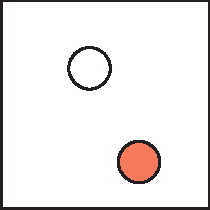
\includegraphics[width=1.5in]{images/samplefigure}
  \caption{Sample illustration.}
\end{figure}


\section{Clamp Design}

\section{Arduino Interface}

\section{UI Design}

\section{Path Generation Algorithm}

\subsection{Constraint Generation}

\subsection{Heuristic Ordering}

\subsection{Polyline Conversion}

\section{YouBot Control}

\subsection{Arm Control}

\subsection{Base Control}

\section{YouBot Planning and Collision Avoidance}

\section{Results}

\section{Conclusion}

\subsection{Future Work}



\section*{Acknowledgements}

Mehmet Dogar and Robert Katzschmann, for suggestions for fixing the YouBot arm control when it wasn't working, which still didn't work.

\section{References}
To Cite:
Ikeabot for example for hand tools for the YouBot.


\bibliographystyle{acmsiggraph}
\bibliography{template}
\end{document}
